% This is LLNCS.DEM the demonstration file of
% the LaTeX macro package from Springer-Verlag
% for Lecture Notes in Computer Science,
% version 2.4 for LaTeX2e as of 16. April 2010
%
\documentclass{llncs}

% allows for temporary adjustment of side margins
\usepackage{chngpage}

% just makes the table prettier (see \toprule, \bottomrule, etc. commands below)
\usepackage{booktabs}

\usepackage[utf8]{inputenc}

% URL handling
\usepackage{url}
\urlstyle{same}

% footnotes
\usepackage{scrextend}

% Todos
%\usepackage[colorinlistoftodos]{todonotes}
%\newcommand{\ke}[1]{\todo[size=\small, color=orange!40]{\textbf{Kai:} #1}}
%\newcommand{\tb}[1]{\todo[size=\small, color=green!40]{\textbf{Thomas:} #1}}


%\usepackage{makeidx}  % allows for indexgeneration

%\usepackage{amsmath}
\usepackage{amsmath, amssymb}
\usepackage{mathabx}

% monospace within text
\newcommand{\ms}[1]{\texttt{#1}}

%\usepackage{listings}% http://ctan.org/pkg/listings
%\lstset{
  %numbers=left,numbersep=2mm,frame=single,mathescape,fontsize=\scriptsize
%}

% examples
\usepackage{fancyvrb}
\DefineVerbatimEnvironment{ex}{Verbatim}{numbers=left,numbersep=2mm,frame=single,fontsize=\scriptsize}

\newenvironment{gcotable-1}{
  \scriptsize
  \sffamily
  \vspace{0.3cm}
  \begin{tabular}{l|l|l|l|l|l}
  \hline
  \textbf{c. type} & \textbf{context concept} & \textbf{p. list} & \textbf{concepts} & \textbf{c. element} & \textbf{c. value} \\
  \hline

}{
  \hline
  \end{tabular}
  \linebreak
}

\newenvironment{gcotable}{
  \scriptsize
  \sffamily
  \vspace{0.3cm}
	\begin{center}
  \begin{tabular}{l|l|l|l|l|l|l}
  \hline
  \textbf{c. type} & \textbf{context class} & \textbf{left p. list} & \textbf{right p. list} & \textbf{classes} & \textbf{c. element} & \textbf{c. value} \\
  \hline

}{
  \hline
  \end{tabular}
	\end{center}
}

\newenvironment{DL}{
  %\scriptsize
  %\sffamily
  \vspace{0.3cm}
	\begin{center}
  \begin{tabular}{r l}

}{
  \end{tabular}
	\end{center}
}

\newenvironment{evaluation}{
  %\scriptsize
  %\sffamily
  \vspace{0.3cm}
	\begin{center}
  \begin{tabular}{l|c|c|c|c|c|c}
  \hline
  \textbf{Constraint Class} & \textbf{DSP} & \textbf{OWL2-DL} & \textbf{OWL2-QL} & \textbf{ReSh} & \textbf{ShEx} & \textbf{SPIN} \\
  \hline

}{
  \hline
  \end{tabular}
	\end{center}
}

\newenvironment{evaluation-generic-overview}{
  %\scriptsize
  %\sffamily
  %\vspace{0.3cm}
	\begin{center}
  \begin{tabular}{l|c|c}
  \hline
  \textbf{Constraint Classes} & \textbf{\#} & \textbf{\%} \\
  \hline

}{
  \hline
  \end{tabular}
  %\linebreak
	\end{center}
}

\usepackage{xspace}
% Einfache und doppelte Anfuehrungszeichen
\newcommand{\qs}{``} 
\newcommand{\qe}{''\xspace} 
\newcommand{\sqs}{`} 
\newcommand{\sqe}{'\xspace} 

% checkmark
\usepackage{tikz}
\def\checkmark{\tikz\fill[scale=0.4](0,.35) -- (.25,0) -- (1,.7) -- (.25,.15) -- cycle;} 

% Xs
\usepackage{pifont}

% Tabellenabstände kleiner
\setlength{\intextsep}{10pt} % Vertical space above & below [h] floats
\setlength{\textfloatsep}{10pt} % Vertical space below (above) [t] ([b]) floats
% \setlength{\abovecaptionskip}{0pt}
% \setlength{\belowcaptionskip}{0pt}

\usepackage{tabularx}
\newcommand{\hr}{\hline\noalign{\smallskip}} % für die horizontalen linien in tabellen

% pipe
%\usepackage[T1]{fontenc}

% Todos
\usepackage[colorinlistoftodos]{todonotes}
\newcommand{\ke}[1]{\todo[size=\small, color=orange!40]{\textbf{Kai:} #1}}
\newcommand{\tb}[1]{\todo[size=\small, color=green!40]{\textbf{Thomas:} #1}}

\setcounter{secnumdepth}{5}

\begin{document}

%
%
\title{Formulating and Validating RDF Constraints Generically}
%\subtitle{}
%
\titlerunning{XXXXX}  % abbreviated title (for running head)
%                                     also used for the TOC unless
%                                     \toctitle is used
%
\author{Thomas Bosch\inst{1} \and X\inst{2} \and X\inst{2} \and X\inst{2} \and Kai Eckert\inst{2}}
%
\authorrunning{XXXXX} % abbreviated author list (for running head)
%
%%%% list of authors for the TOC (use if author list has to be modified)
\institute{GESIS – Leibniz Institute for the Social Sciences, Germany\\
\email{thomas.bosch@gesis.org},\\ 
\and
University of Mannheim, Germany \\
\email{\{kai\}@informatik.uni-mannheim.de} 
}

\maketitle              % typeset the title of the contribution

\begin{abstract}

For XML, XML Schema is the standard constraint language to validate XML documents.
For RDF, however, there are multiple candidates for languages to express constraints on RDF data - but there is no standard language for RDF validation.
W3C and DCMI working groups on RDF validation identified requirements to formulate and to validate RDF constraints.
The majority of these constraints can be represented in description logics providing a logical underpinning of these constraints.
We developed an ontology describing any RDF constraint generically (whether expressible in description logics or not).
In parallel, we defined a basic terminology and a classification system for RDF constraints.

A constraint (expressed by constraint language \ms{$sc_{\alpha}$}) can be transformed to a constraint (expressed by constraint language \ms{$sc_{\beta}$}) by using the RDF constraint ontology as intermediate language. 
Currently, we cannot validate every constraint language or constraint of a constraint language.
If we define a validation for a constraint generically and if we map semantically equivalent constraints (expressed by different constraint languages) to that generically expressed constraint, we are able to provide the validation of these constraints out of the box.

\keywords{RDF Validation, RDF Constraints, RDF Validation Requirements, Transformation, Linked Data, Semantic Web}
\end{abstract}
%

% ---------------

\section{Introduction}

For many RDF applications, the formulation of constraints and the automatic validation of data according to these constraints is a much sought-after feature. 
In 2013, the W3C invited experts from industry, government, and academia to the RDF Validation Workshop\footnote{\url{http://www.w3.org/2012/12/rdf-val/}}, 
where first use cases have been presented and discussed. 
Two working groups (WGs),  that follow up on this workshop and address RDF constraint formulation and validation, are established in 2014: 
the W3C RDF Data Shapes WG\footnote{\url{http://www.w3.org/2014/rds/charter}} and the DCMI RDF Application Profiles WG\footnote{\url{http://wiki.dublincore.org/index.php/RDF-Application-Profiles}}. 

Bosch and Eckert \cite{BoschEckert2014} initiated a database on RDF validation requirements to collect case studies, use cases and especially requirements regarding RDF validation collaboratively and in a comprehensive and structured way. 
%\er{Just for reminding ourselves:  being careful using what is a use-case and what is a case-study later in the text.(http://www.w3.org/2001/sw/sweo/public/UseCases/)}
%\tb{agreed, will take care}
This database is continuously updated and openly available at \url{http://purl.org/net/rdf-validation}. It is used to evaluate and compare several existing solutions for RDF constraint formulation and validation. 
The requirements are classified to provide a high-level view on different solutions and to facilitate a better understanding of the problem domain \cite{BoschEckert2014}.  
Each requirement to formulate RDF constraints is directly mapped to an RDF constraint.

There are multiple constraint languages with different syntaxes and semantics which can be used to express RDF constraints, e.g., \emph{at-least} restrictions.
The most promising ones on being the standard, are
the SPARQL Inferencing Notation (SPIN)\footnote{\url{http://spinrdf.org/}}, 
the Web Ontology Language (OWL 2)\footnote{\url{http://www.w3.org/TR/owl2-syntax/}}, 
Shape Expressions (ShEx)\footnote{\url{http://www.w3.org/Submission/shex-primer/}}, 
Resource Shapes (ReSh)\footnote{\url{http://www.w3.org/Submission/shapes/}}, 
and Description Set Profiles (DSP)\footnote{\url{http://dublincore.org/documents/2008/03/31/dc-dsp/}}.
However, there is no single standard general-purpose constraint language.
The choice depends on the individual use case.

\tb{introduction copied from first paper - need to be modified}

%\section{Ideas}

%constraint design patterns:
% - ontology design pattern.org
% - DSP uses other design pattern
% - constraint elements are the same / 
% - constraint / constraint elements / constraint design patterns / constraint language

%dependency between requirements / when this requirements is fulfilled then this is also fulfilled (e.g. min card and requ. car)
%min car more powerful than req. propery

\section{Motivation}

Cardinality restrictions can be expressed either generically by description logics (DL) (\ms{generic constraints}) and additional constraints or specifically (\ms{specific constraints}) by domain-specific constraint languages such as OWL 2, DSP, ShEx, ReSh, and SPIN.
With minimum qualified cardinality restrictions we can state, e.g., that a star fleet captain commands at least one vessel, which may be represented by DL in a logical way:

\begin{DL}
$StarFleetCaptain \sqsubseteq \geq1 commandsVessel . Vessel $
\end{DL}

The same constraint may also be represented by different constraint languages like OWL 2, ShEx, ReSh, or DSP:

\begin{ex}
# OWL 2
# -----
StarFleetCaptain
    a owl:Restriction ;
    owl:minQualifiedCardinality 1 ;
    owl:onProperty commandsVessel ;
    owl:onClass Vessel .
		
# ShEx
# ----
StarFleetCaptain { commandsVessel @Vessel{1, } }

# ReSh
# ----
StarFleetCaptain a rs:ResourceShape ; rs:property [
    rs:name "commandsVessel" ; rs:propertyDefinition commandsVessel ;
    rs:valueShape Vessel ;
    rs:occurs rs:One-or-many ; ] .
				
# DSP
# ---			
descriptionTemplate a dsp:DescriptionTemplate ; 
    dsp:resourceClass StarFleetCaptain ; 
    dsp:statementTemplate [ a dsp:NonLiteralStatementTemplate ;
        dsp:minOccur 1 ; dsp:maxOccur "infinity" ; 
        dsp:property commandsVessel ; 
        dsp:nonLiteralConstraint [ a dsp:NonLiteralConstraint ;
            dsp:valueClass Vessel ] ] .
\end{ex}

As \ms{Janeway} commands the vessel \ms{Voyager} (\ms{commandsVessel(Janeway,Voyager)}) and \ms{Voyager} is defined to be a \ms{Vessel} (\ms{rdf:type(Voyager,Vessel)}), the assignment of \ms{Janeway} to the class \ms{StarFleetCaptain} (\ms{rdf:type(Janeway,StarFleetCaptain)}) does not cause any constraint violation.
A constraint violation is raised, however, when there is no \ms{commandsVessel} relationship pointing from the individual \ms{Janeway}. 
A constraint violation is also raised, when there is a triple \ms{commandsVessel(Janeway,Voyager)}, but \ms{Voyager} is not explicitly defined to be a \ms{Vessel}, 
i.e. the triple \ms{rdf:type(Voyager,Vessel)} is not present in the data. 
As the object of the \ms{commandsVessel} property is assigned to another class than \ms{Vessel}, 
the triples \ms{commandsVessel(Sisko,DS9)}, \ms{rdf:type(Sisko,StarFleetCaptain)}, and \ms{rdf:type(DS9,SpaceStation)}  
also cause a constraint violation.

As there is no standard constraint language, constraint designers may choose different constraint languages to express the identical cardinality restriction. 
When constraint designers choose one constraint language to express an arbitrary constraint, it should be possible to transform this constraint into a constraint expressed by any other constraint language. 
This is important as it is often the case that one constraint designer knows to read and to write constraints in one constraint language very well but not in another constraint language. 
This way, constraint designers may communicate with each other without the necessity to understand all constraint languages and the interoperability of constraint languages is enhanced.


There are validation environments available enabling to automatically validate RDF constraints expressed by just a few constraint languages such as OWL 2\footnote{\url{purl.org/net/rdfval-demo}\label{footnote1}}, DSP\footref{footnote1}, and ShEx\footnote{\url{http://www.w3.org/2013/ShEx/FancyShExDemo}}.
It should be possible to validate any RDF constraints expressed by any constraint language automatically and what is even more important in exactly the same manner without any differences.  

The following table shows the mapping between the cardinality restriction expressed in DL and the cardinality restriction (\ms{generic constraint}) expressed by a generic constraint language conforming to an ontology to describe any RDF constraint generically (see section~\ref{sec:ontology}).
Each constraint is either a constraint on classes or a constraint on properties.

\begin{gcotable}
property & Captain & commandsVessel & - & Vessel & $\geq$ & 1 \\
\end{gcotable}

The cardinality restriction (expressed by the generic constraint language) is represented in RDF as follows:

\begin{ex}
[   a PropertyConstraint ;
    contextClass StarFleetCaptain ;
    leftProperties ( commandsVessel ) ;
    classes ( Vessel ) ;
    constrainingElement ">=" ;
    constrainingValue "1" ] .
\end{ex}

We implemented the automatic validation for the cardinality restriction expressed by the generic constraint language within our SPIN validation environment (see SPARQL query above):

\begin{ex}
[   a PropertyConstraint ;
    contextClass ?cc ;
    leftProperties ( ?p1 ) ;
    classes ( ?c1 ) ;
    constrainingElement ">=" ;
    constrainingValue ?cv ] .
		
?subject rdf:type ?cc .

BIND ( qualifiedCardinality( ?subject, ?p1, ?c1 ) AS ?c ) .
FILTER ( ?c < ?cv ) .		  
\end{ex}

If we transform a specific constraint (expressed by any constraint language) into a generic constraint (expressed by the generic constraint language), we will be able to validate the generic constraint and therefore the specific constraint immediately. 
As a consequence, we do not have to specify an automatic validation for each specific constraint, as we need to define an automatic validation only once for each generic constraint. 
We have to provide an automatic validation for each generic constraint in order to support the automatic validation for each specific constraint.

When domain experts use graphical user interfaces to define constraints in a user-friendly way (without the necessity to express constraints on their own), 
constraints can be mapped to either a specific or a generic constraint, as for both an automatic validation is provided in the background.    
So, the user does not have to know how to express specific constraints using any constraint language.
If there is a new constraint not covered by any existing constraint language, one can just define the automatic validation for a corresponding generic constraint.
This way, one is able to extend existing constraint languages and also to define new constraint languages if existing constraint languages are not sufficient to express particular constraints.
If a language designer develops a new constraint language, 
the language designer only needs to define a mapping between the new constraint language and the generic constraint language
in order to be able to automatically validate the constraints expressible by the new constraint language.

The \textbf{contributions} of this paper are:
\begin{itemize}
	%\item Any specific constraint (expressed by any constraint language) can be transformed into a generic constraint (expressed by the generic constraint language)
	%\item Any specific constraint (expressed by any constraint language A) can be transformed into any specific constraint (expressed by any constraint language B)
	%\item Any specific constraint (expressed by any constraint language) can be validated automatically (if an automatic validation is defined only once for corresponding generic constraint)
	\item We define a basic terminology and classification system for RDF constraints
	\item We developed an ontology describing any RDF constraint generically (whether expressible in DL or not)%which can also be expressed by any constraint language
	%\item We present that any RDF constraint can be described by the developed ontology - whether the constraint can be expressed in DL or not 
	\item We show how to transform specific constraints (expressed by any constraint language A) into generic constraints and into specific constraints (expressed by any other constraint language B)
  \item We explain that any specific constraint can be validated automatically (if an automatic validation is defined only once for the corresponding generic constraint)
\end{itemize}

%The \textbf{benefits} of our framework are:
%\begin{itemize}
	%\item Any specific constraint (expressed by any constraint language) can be transformed into a generic constraint (expressed by the generic constraint language)
	%\item Any specific constraint (expressed by any constraint language A) can be transformed into any specific constraint (expressed by any constraint language B)
	%\item Any specific constraint (expressed by any constraint language) can be validated automatically (if an automatic validation is defined only once for corresponding generic constraint)
%\end{itemize}

\textcolor{red}{paper organization}

\section{RDF Constraints Ontology} 
\label{sec:ontology}

In order to define this ontology to describe RDF constraints generically, it is needed to define the terminology for the formulation of constraints. 
A \ms{constraint language} is a language which is used to formulate constraints.
The W3C Data Shapes WG defines \ms{constraint} as a component of a schema what needs to be satisfied\footnote{\url{https://www.w3.org/2014/data-shapes/wiki/Glossary}}.
We identified four dimensions to classify constraints:
\begin{itemize}
  \item \ms{Universality:} specific constraints vs. generic constraints
	\item \ms{Complexity:} simple constraints vs. complex constraints
	\item \ms{Context:} property constraints vs. class constraints
	\item \ms{DL Expressivity:} constraints expressible in DL vs. constraints not expressible in DL
\end{itemize}

As there are already five promising constraint languages, our purpose is not to invent a new constraint language.
We developed a very simple ontology (only three classes, three object properties, and three data properties) which is universal enough to describe any RDF constraint expressible by any RDF constraint language (see the conceptual model in figure \ref{fig:RDF-CO-conceptual-model}).
We call this ontology the \ms{RDF constraints ontology (RDF-CO)}\footnote{Available at: \url{https://github.com/boschthomas/RDF-constraints-ontology}}.

\begin{figure}
	\centering
		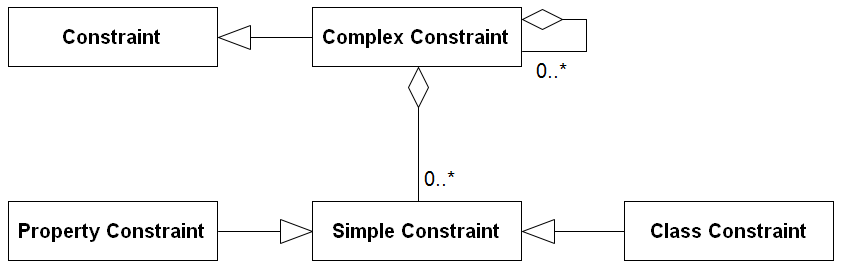
\includegraphics[width=0.80\textwidth]{images/RDF-CO-conceptual-model.png}
	\caption{RDF constraints ontology (RDF-CO) - conceptual model}
	\label{fig:RDF-CO-conceptual-model}
\end{figure}

\ms{Specific constraints} are expressed by specific constraint languages like DSP, OWL 2, ReSh, ShEx, and SPIN.
\ms{Generic constraints} are expressed by the RDF-CO.
As RDF-CO describes constraints generically, RDF-CO does not distinguish constraints according to the dimension \ms{universality}. 
The majority of constraints can be expressed in DL (see section \ref{sec:evaluation}).
In contrast, there are constraints which cannot be expressed in DL, but are also representable by the RDF-CO. 
\ms{Complex constraints} encompass \ms{simple constraints} (atomic constraints) and/or further complex constraints.
DL statements representing complex constraints are created out of DL statements representing composed constraints (if expressible in DL). 
Simple constraints may be applied to either properties \ms{properties constraints} or classes \ms{class constraints}.
There are no terms representing simple and complex constraints in the RDF-CO, since context classes (associated simple constraints hold for individuals of these classes) of simple constraints may just be reused by further constraints.
As a consequence, the distinction of property and class constraints is sufficient to describe all possible RDF constraints.

\subsection{Simple Constraints (Expressible in DL)}

Sub-classes of \ms{simple constraints} are \ms{property constraints} and \ms{class constraints} (see the RDF-CO implementation model in figure \ref{fig:RDF-CO-implementation-model}). 
For both property and class constraints a context class, a list of classes, the constraining element, and the constraining value can be stated. 
Lists of left and right properties can only be stated for property constraints.

\begin{figure}
	\centering
		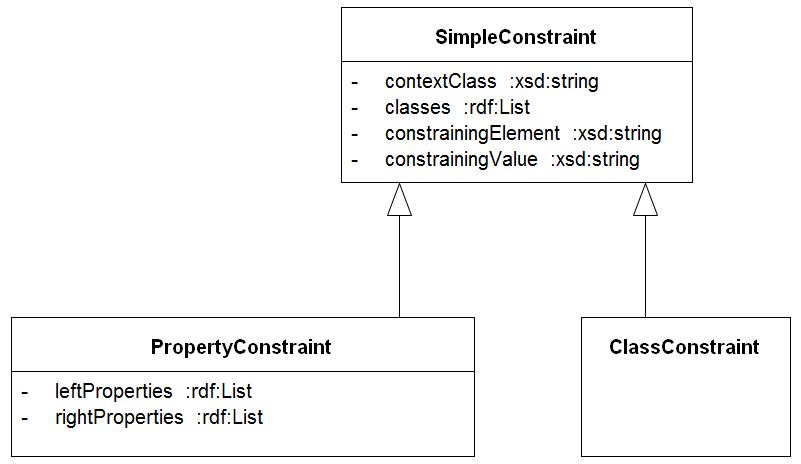
\includegraphics[width=0.70\textwidth]{images/RDF-CO-implementation-model.png}
	\caption{RDF constraints ontology (RDF-CO) - implementation model}
	\label{fig:RDF-CO-implementation-model}
\end{figure}

A constraint holds for all individuals of a context class (\ms{contextClass}).
Consider, e.g., the following cardinality restriction on the property \ms{commandsVessel}, which restricts that a captain must command at least one vessel: 
\begin{DL}
$Captain \sqsubseteq \geq1 commandsVessel . Vessel $
\end{DL}
Mapped to the GCLO the cardinality restriction is classified as a property constraint which holds for individuals of the class \ms{Captain} - the context class:
\begin{gcotable}
property & Captain & commandsVessel & - & Vessel & $\geq$ & 1 \\
\end{gcotable}
The constraining element (\ms{constrainingElement}) is the operator indicating the actual type of constraint like DL concept and role constructors, (in)equality, and further keywords for constrains which cannot be expressed in DL (e.g. regular expressions, constraining facets).
In some cases, a constraint is only complete when in addition to the constraining element a constraining value (\ms{constrainingValue}) is stated.
The cardinality restriction 
\begin{DL}
$\geq$1 commandsVessel . Vessel
\end{DL}
constructs an anonymous class of all individuals who command at least one vessel.
Thus, the constraining element of this property constraint is the DL at-least restriction \ms{$\geq$} and the constraining value is \ms{1}.
\ms{Classes} indicate the list of classes constraints refer to.
In case of the property constraint above, the qualified cardinality restriction refers to the class \ms{Vessel}, 
i.e., restricting the objects, the property \ms{commandsVessel} point to, to be of the class \ms{Vessel}.

\subsection{Simple Constraints (Not Expressible in DL)}

There are simple constraints which cannot be expressed by DL such as literal pattern matching, literal value comparison, literal ranges, default values, and language tag cardinality \cite{BoschNolleAcarEckert2015}.

% maybe additional constraint default values:
% ear shape of races, e.g. vulcans / teeth color
% mathematical operations

There are multiple use cases associated with the requirement to match literals according to given patterns (\ms{Literal Pattern Matching} constraint).
The enterprise vessel, e.g.,  can only have the registry numbers "NCC-1701", "NCC-1701-A", "NCC-1701-B", "NCC-1701-C", "NCC-1701-D", or "NCC-1701-E".
The universal restriction part of this complex constraint can be expressed by OWL 2 DL:
\ms{Enterprise $\sqsubseteq$ $\forall$ registryNumber.RegistryNumber}.
The restriction of the datatype \ms{RegistryNumber}, however, cannot be expressed in DL, but OWL 2 DL can be used anyway to express the literal pattern matching constraint:

\begin{ex}
RegistryNumber
    a rdfs:Datatype ;
    owl:equivalentClass [
        a rdfs:Datatype ;
        owl:onDatatype xsd:string ;
        owl:withRestrictions ( 
            [ xsd:pattern "NCC-1701([-][A-E])?" ] ) ] .
\end{ex}

The second axiom defines \ms{RegistryNumber} as an abbreviation for a datatype restriction on \ms{xsd:string}. 
The first axiom explicitly declares \ms{RegistryNumber} to be a datatype. 
The datatype \ms{RegistryNumber} can be used just like any other datatype like in the universal restriction above.
The literal pattern matching constraint validates \ms{RegistryNumber} literals according to the stated regular expression causing a constraint violation for the triples 
\ms{Janeway commandsEnterprise Voyager} and \ms{Voyager registryNumber "NCC-74656"\textasciicircum{}\textasciicircum{}RegistryNumber}, 
but not for the triples \ms{Picard commandsEnterprise Enterprise} and \ms{Enterprise registryNumber "NCC-1701-E"\textasciicircum{}\textasciicircum{}RegistryNumber}.
The universal restriction and the literal pattern matching constraint are mapped to the generic constraint language as follows:

\begin{gcotable}
property & Enterprise & registryNumber & - & RegistryNumber & $\forall$ & - \\
class & RegistryNumber & - & - & xsd:string & regex & 'NCC-1701([-][A-E])?' \\
\end{gcotable}

The \ms{Literal Pattern Matching} constraint introduces a new constraining element: \ms{regex}.
For this new constraining element, an automatic validation must be implemented in SPIN.
This has to be done once for each constraint which cannot be expressed in DL.

\subsection{Complex Constraints}

\ms{Complex constraints} encompass simple constraints and/or complex constraints.
\textbf{Context-Specific Exclusive OR of Property Groups}\footnote{corresponds to R-13-DISJOINT-GROUP-OF-PROPERTIES-CLASS-SPECIFIC}\textbf{.}
Exclusive or is a logical operation that outputs true whenever both inputs differ (one is true, the other is false).
Only one of multiple property groups should be present in the data.
Half-Klingons, e.g., either have a klingon mother and a human father or a human mother and a klingon father, which can be expressed by ShEx:

\begin{ex}
Half-Klingon { 
    ( klingonMother Klingon , humanFather Human ) |
    ( humanMother Human , klingonFather Klingon ) }
\end{ex}

As \ms{B'Elanna Torres} is a \ms{Half-Klingon} with a klingon mother and a human father, this data is valid:

\begin{ex}
BElannaTorres a Half-Klingon ;
    klingonMother Miral ; humanFather JohnTorres .
\end{ex}

%\begin{DL}
%rdf:type(BElannaTorres,Half-Klingon) \\
%klingonMother(BElannaTorres,Miral) \\
%klingonMother(BElannaTorres,JohnTorres)
%\end{DL}

This complex constraint can be mapped to DL:

\begin{DL}
Half-Klingon $\sqsubseteq$ ($\neg$E $\sqcap$ F) $\sqcup$ (E $\sqcap$ $\neg$F) \\ 
E $\equiv$ A $\sqcap$ B \\
F $\equiv$ C $\sqcap$ D \\
A $\sqsubseteq$ $\geq$ 1 klingonMother.Klingon $\sqcap$ $\leq$ 1 klingonMother.Klingon \\
B $\sqsubseteq$ $\geq$ 1 humanFather.Human $\sqcap$ $\leq$ 1 humanFather.Human \\
C $\sqsubseteq$ $\geq$ 1 humanMother.Human $\sqcap$ $\leq$ 1 humanMother.Human \\
D $\sqsubseteq$ $\geq$ 1 klingonFather.Klingon $\sqcap$ $\leq$ 1 klingonFather.Klingon \\
\end{DL}

The constraint expressed by DL can be mapped to a generic constraint:

\begin{gcotable}
class & Half-Klingon & - & - & $\neg$E $\sqcap$ F, E $\sqcap$ $\neg$F & $\sqcup$ & - \\
class & $\neg$E $\sqcap$ F & - & - & $\neg$E, F & $\sqcap$ & - \\
class & E $\sqcap$ $\neg$F & - & - & E, $\neg$F & $\sqcap$ & - \\
class & $\neg$E & - & - & E & $\neg$ & - \\
class & E & - & - & A, B & $\sqcap$ & - \\
class & $\neg$F & - & - & F & $\neg$ & - \\
class & F & - & - & C, D & $\sqcap$ & - \\
class & A & - & - & A1, A2 & $\sqcap$ & - \\
property & A1 & klingonMother & - & Klingon & $\geq$ & 1 \\
property & A2 & klingonMother & - & Klingon & $\leq$ & 1 \\
class & B & - & - & B1, B2 & $\sqcap$ & - \\
property & B1 & humanFather & - & Human & $\geq$ & 1 \\
property & B2 & humanFather & - & Human & $\leq$ & 1 \\
class & C & - & - & C1, C2 & $\sqcap$ & - \\
property & C1 & humanMother & - & Human & $\geq$ & 1 \\
property & C2 & humanMother & - & Human & $\leq$ & 1 \\
class & D & - & - & D1, D2 & $\sqcap$ & - \\
property & D1 & klingonFather & - & Klingon & $\geq$ & 1 \\
property & D2 & klingonFather & - & Klingon & $\leq$ & 1 \\
\end{gcotable}

Even though, tools may generate generic constraints automatically, this complex constraint is composed of many other complex (e.g. minimum and maximum qualified cardinality restrictions) and simple constraints (e.g. constraints on sets).
As \ms{exact (un)qualified cardinality restrictions} and \ms{exclusive or} are frequently used complex constraints,
we propose using them as simple constraints - 	in terms of syntactic sugar.
As a consequence, the \ms{Context-Specific Exclusive OR of Property Groups} constraint above is represented as a generic constraint more intuitively and concisely:

\begin{gcotable}
class & Half-Klingon & - & - & E, F & XOR \\
class & E & - & - & A, B & $\sqcap$ \\
class & F & - & - & C, D & $\sqcap$ \\
property & A & klingonMother & - & Klingon & = & 1 \\
property & B & humanFather & - & Human & = & 1 \\
property & C & humanMother & - & Human & = & 1 \\
property & D & klingonFather & - & Klingon & = & 1 \\
\end{gcotable}

\subsection{Simple Constraints (Syntactic Sugar)}

Almost 15 percent of all RDF constraints are complex constraints which can be simplified and therefore formulated as simple constraints when used in terms of syntactic sugar (see section \ref{sec:evaluation}).

There three forms of RBox axioms: role inclusions, role equivalences and role disjointness. 
OWL provides a variety of others, namely role transitivity, symmetry, asymmetry, reflexivity and irreflexivity. 
These are sometimes considered as basic axiom types in DLs as well, using some suggestive notation such as
\ms{Trans(ancestorOf)} to express that the role ancestorOf is transitive. 
However, such axioms are just syntactic sugar; 
all role characteristics can be expressed using the basic features of DLs.
\ms{Irreflexive Object Properties}\footnote{corresponds to the requirement \ms{R-60-IRREFLEXIVE-OBJECT-PROPERTIES}}
restricts that an object property is irreflexive if it is never locally reflexive, i.e. no individual is connected by the object property to itself \cite{Kroetzsch2012}.
Irreflexivity constraints, stating that individuals cannot be married to themselves, can be represented in DL:

\begin{DL}
$\top$ $\sqsubseteq$ $\neg$ $\exists  marriedTo . Self$
\end{DL}

When mapped to the RDF-CO, the complex constraint aggregates three simple constraints (one property and two class constraints):

\begin{gcotable}
property & $\exists$ marriedTo . Self & marriedTo & - & Self & $\exists$ & - \\
class & $\neg$ $\exists$ marriedTo . Self & - & - & $\exists$ marriedTo . Self & $\neg$ & - \\
class & $\top$ & - & - & $\top$, $\neg$ $\exists$ marriedTo . Self & $\sqsubseteq$ & - \\
\end{gcotable}

When using the RBox axiom \ms{role irreflexivity} as syntactic sugar, 
the complex constraint transforms into a simple property constraint with exactly the same semantics:

\begin{gcotable}
property & $\top$ & marriedTo & - & - & irreflexive & - \\
\end{gcotable}

The \ms{Primary Key Properties} constraint is often useful to declare a given (datatype) property as the "primary key" of a class, so that the system can enforce uniqueness. 
Starfleet officers are uniquely identified by their command authorization code (e.g. to activate and cancel auto-destruct sequences).
It means that the property \ms{commandAuthorizationCode} is inverse functional - mapped to DL and RDF-CO as follows:

\begin{DL}
$(\ms{funct } commandAuthorizationCode\sp{\overline{\ }})$
\end{DL}

\begin{gcotable}
property & $\top$ & commandAuthorizationCode$^{-}$ & commandAuthorizationCode & - & inverse & - \\
property & $\top$ & commandAuthorizationCode$^{-}$ & - & - & functional & - \\
\end{gcotable}

Keys are even more general, i.e., a generalization of inverse functional properties\footnote{\url{http://www.w3.org/TR/2012/REC-owl2-rdf-based-semantics-20121211/#Semantic_Conditions_for_Keys}}.
A key can be a datatype property, an object property, or a chain of properties.
For this generalization purposes, as there are different sorts of key, and as keys can lead to undecidability, 
DL is extended with \ms{key boxes} and a special \ms{keyfor} construct\cite{Lutz2005}.
This leads to the following DL and RDF-CO mappings (only one simple property constraint) for the example:

\begin{DL}
commandAuthorizationCode \ms{keyfor} StarfleetOfficer
\end{DL}

\begin{gcotable}
property & StarFleetOfficer & commandAuthorizationCode & - & - & keyfor & - \\
\end{gcotable}

%\begin{itemize}
  %\item domain and range
	%\item Primary Key Properties
	%\item ( Exact Qualified Cardinality Restrictions on Properties )
%\end{itemize}

%\subsection{Disjoint Classes}
%
%\begin{DL}
%Hologram $\sqcap$ Human $\sqsubseteq$ $\perp$\\
%Alternative:\\
%$Hologram \sqsubseteq \neg Human$
%\end{DL}
%
%\subsection{Minimum Qualified Cardinality Restrictions on Properties}
%
%\begin{DL}
%$FederationCaptain \sqsubseteq Federation \sqcap \geq1 commandsVessel . Vessel $
%\end{DL}

%\section{Transformations and Automatic Validation of Specific Constraints}
%\section{Transformations between Specific Constraints (Expressed by Different Constraint Languages)}
\section{Transformations between Specific Constraints}
\label{sec:transformations}

RDF data providers ensure that their data conforms to constraints which are part of the contract between the providers and the consumers of that data.
As there is no standard way, these constraints may be represented by multiple constraint languages (there are even more than the five promising ones)\footnote{i.a. Bibframe, DQTP, Pellet ICV, RDFUnit, SPARQL, Stardog ICV}.
There is an obvious need to transform a specific constraint (\ms{$sc_{\alpha}$}) (expressed by any constraint language \ms{$\alpha$}) into a specific constraint (\ms{$sc_{\beta}$}) (expressed by any constraint language \ms{$\beta$}) - when they have the same semantics.
We use the RDF-CO as intermediate language for these transformations.
If we define mappings ($m(sc_{\alpha}), m(sc_{\beta})$) from these two specific constraints to the corresponding generic constraint (\ms{gc}),
we can convert them automatically:

\begin{DL}
$ gc = m(sc_{\alpha}) = m(sc_{\beta}) $
\end{DL}

We do not need to define mappings for each pair of semantically equivalent specific constraint.
Let's assume we are able to express a constraint by 5/6/7/8/9/10 constraint languages.
Without the intermediate generic constraint, we would have to define one mapping for each pair of specific constraints expressed by a specific constraint language
- that are \ms{\( {n \choose 2} \)} mappings for each constraint (example: 10/15/21/28/36/45).
With an intermediate generic constraint, we only need to define \ms{n} mappings from the specific constraints to the generic constraint (example: 5/6/7/8/9/10 ).

%(n(n+1))/2

%\begin{DL}
%\(\sum \limits_{i=1}^n i = \frac{n(n+1)}{2}\)
%\(\sum \limits_{i=1}^n i\)
%\(\Binom{n}{2} \)
%\( {n \choose 2} \)
%\end{DL}

\ms{Allowed Values}\footnote{corresponds to the requirements \ms{R-30-ALLOWED-VALUES-FOR-RDF-OBJECTS} and \ms{R-37-ALLOWED-VALUES-FOR-RDF-LITERALS}}
is a common requirement to narrow down the value space of a property by an exhaustive enumeration of the valid values (both literals or resources). 
The Enterprise, e.g., is only commanded by the captains Archer, Kirk, and Picard.
This complex constraint is composed of the two simple constraints \ms{universal quantification} and \ms{allowed values} which can be represented in DL:

%\begin{DL}
%StarfleetCaptain $\equiv$ $\forall$ overruledBy . \{Commodore\} $\sqcup$ \{Admiral\}
%\end{DL}

\begin{DL}
Enterprise $\equiv$ $\forall$ commandedBy . \{Archer\} $\sqcup$ \{Kirk\} $\sqcup$ \{Picard\}
\end{DL}

First, we map these DL statements to two simple constraints corresponding to the RDF-CO (we define the class \ms{EnterpriseCaptains} by simply enumerating its instances):

%\begin{gcotable}
%property & StarfleetCaptain & overruledBy & - & CaptainOverruler & $\forall$ & - \\
%class & CaptainOverruler & - & - & \{Commodore\},\{Admiral\} & $\sqcup$ & - \\
%\end{gcotable}

\begin{gcotable}
property & Enterprise & commandedBy & - & EnterpriseCaptains & $\forall$ & - \\
class & EnterpriseCaptains & - & - & \{Archer\},\{Kirk\},\{Picard\} & $\sqcup$ & - \\
\end{gcotable}

The next step is to define one mapping for each specific constraint to the generic constraint.
The specific constraints (\ms{$sc_{OWL 2}$}, \ms{$sc_{ReSh}$}, and \ms{$sc_{ShEx}$}) expressed by OWL 2, ReSh, and ShEx look like this:

\begin{ex}
# OWL 2:
Enterprise rdfs:subClassOf [ a owl:Restriction .
    owl:onProperty commandedBy .
    owl:allValuesFrom [ a owl:Class ;
        owl:oneOf ( Archer Kirk Picard ) ] ] .
# ReSh:
Enterprise a rs:ResourceShape ; rs:property [
    rs:name "commandedBy" ; rs:propertyDefinition commandedBy ;
    rs:allowedValue Archer , Kirk , Picard ;
    rs:occurs rs:Exactly-one ; ] .
# ShEx:
Enterprise {
    commandedBy (Archer Kirk Picard) }
\end{ex}

%\begin{ex}
%# DSP:
%[ a dsp:DescriptionTemplate ;
    %dsp:resourceClass StarfleetCaptain ; 
    %dsp:statementTemplate [ a dsp:NonLiteralStatementTemplate ; 
        %dsp:property overruledBy ; 
        %dsp:nonLiteralConstraint [ a dsp:NonLiteralConstraint ;
            %dsp:valueClass Commodore , Admiral ] ] ] .
%# OWL 2:
%StarfleetCaptain rdfs:subClassOf [ a owl:Restriction .
    %owl:onProperty overruledBy .
    %owl:allValuesFrom [ a owl:Class ;
        %owl:oneOf ( Commodore Admiral ) ] ] .
%# ReSh:
%%StarfleetCaptain a rs:ResourceShape ;
    %%rs:property [
        %%rs:name "overruledBy" ; rs:propertyDefinition overruledBy ;
        %%rs:valueShape Commodore ; rs:occurs rs:Zero-or-many ; ] ;
    %%rs:property [
        %%rs:name "overruledBy" ; rs:propertyDefinition overruledBy ;
        %%rs:valueShape Admiral ; rs:occurs rs:Zero-or-many ; ] ;
%# ShEx:
%:StarfleetCaptain {
    %:overruledBy @:Commodore* , :overruledBy @:Admiral* }
%\end{ex}

\section{Automatic Validation of Specific and Generic Constraints}

We can provide an automatic validation of all specific constraints (expressed by any constraint language) by defining a mapping to SPIN.
That's what we have done for all OWL 2 and DSP constructs (see section \ref{sec:implementation}).
%We do not have to define a mapping to SPIN for each specific constraint. 
%when we define a mapping to SPIN for each generic constraint.
But, if we define a mapping from a specific constraint to the corresponding generic constraint and if we define a mapping from the generic constraint to SPIN,
we do not have to define a mapping to SPIN for that specific constraint - we can perform an automatic validation for the generic and for the specific constraint as well.
As a consequence, we only have to define one SPIN mapping for each constraint corresponding to a requirement within the RDF validation requirements database.
19 of 74 RDF constraints can be expressed by at least four constraint languages \cite{BoschNolleAcarEckert2015}.
This means, that there must be 76 (four for each constraint) implementations to validate  these constraints - instead of only 19 (one for each constraint).

Within our SPIN validation environment, we define a SPIN construct template for each generic constraint\footnote{for details about the SPIN validation environment see \cite{BoschEckert2014-2}}.
The SPIN construct template contains a SPARQL CONSTRUCT query which generates constraint violation triples (\ms{spin:ConstraintViolation}) indicating the subject (\ms{spin:violationRoot}) and the properties (\ms{spin:violationPath}), causing the constraint violation, and the reason why the constraint violation has been raised (\ms{rdfs:label}).
The SPIN construct template creates the constraint violation triples if all triple patterns within the SPARQL WHERE clause match.
The SPARQL CONSTRUCT query for the universal quantification (of the previous example in section \ref{sec:transformations}) is shown below:

\begin{ex}
CONSTRUCT {
    [   a spin:ConstraintViolation ; spin:violationRoot ?subject ;
        rdfs:label ?violationMessage ; spin:violationPath ?p1 . }
WHERE {	  
    [   a gclo:PropertyConstraint ;
        gclo:contextClass ?cc ;
        gclo:leftProperties ( ?p1 ) ;
        gclo:classes ( ?c1 ) ;
        gclo:constrainingElement "universal quantification" ] .
    [   a gclo:ClassConstraint ;
        gclo:contextClass ?c1 ;
        gclo:classes ( ?i1 ?i2 ?i3 ) ;
        gclo:constrainingElement "union" ] .				
    ?subject a ?cc ; ?p1 ?i .
    FILTER ( ?i != ?i1 && ?i != ?i2 && ?i != ?i3 ) . }
\end{ex}

As a consequence, the validation results do not differ for semantically equivalent constraints when they are based on multiple validation implementations, as there is only one validation implementation for each constraint - independent from the used constraint language.

%\subsection{Not Allowed Values}

\section{Implementation}
\label{sec:implementation}

SPARQL is generally seen as the method of choice to validate RDF data according to certain constraints, although it is not ideal for their formulation. 
In contrast, OWL 2 and DSP constraints are comparatively easy to understand, but lack an implementation to validate RDF data. 
Bosch and Eckert\cite{BoschEckert2014-2} use SPIN as basis to define a
validation environment in which the validation of any constraint language\footnote{the only limitation is that constraint languages must be represented in RDF} can be implemented by representing them in SPARQL. 
The validation implementation of constraint languages is fully declarative,
consisting of a mapping from constraint languages to SPIN in form of SPARQL CONSTRUCT queries.
SPIN represents both the SPIN mappings and the SPARQL queries in RDF. 
Within the validation environment, we fully implemented an automatic validation of all OWL 2 DL\footnote{OWL 2 SPIN mapping: \url{https://github.com/boschthomas/OWL2-SPIN-Mapping}} and DSP\footnote{DSP SPIN mapping: \url{https://github.com/dcmi/DSP-SPIN-Mapping}} constructs (for the complete DSP validation see \cite{BoschEckert2014-2}). 
The implementation can be tested at \url{http://purl.org/net/rdfval-demo}.
The SPIN engine checks for each resource if it satisfies all constraints (associated with its assigned classes) and generates a result RDF graph containing information about all constraint violations.

We provide a mapping from the generic constraint language to SPIN\footnote{GCL SPIN mapping: \url{https://github.com/boschthomas/GCL-SPIN-Mapping}} in order to automatically validate each type of generic constraint (simple, complex, property, and class constraints).
Part of future work will be 
\begin{itemize}
	\item to provide a GUI which generates generic constraints automatically according to inputs of domain experts who are not familiar with the formulation of constraints.
	\item to offer bidirectional transformations between specific constraints (expressed by multiple constraint languages) and generic constraints. 
	\item to provide translations between specific constraints (expressed by any specific constraint language) by using generic constraints as an intermediate transformation step.
\end{itemize}

\section{Evaluation}
\label{sec:evaluation}

We evaluated to which extend the most promising five constraint languages fulfill each of the overall 74 requirements to formulate RDF constraints \cite{BoschNolleAcarEckert2015}.
If a constraint can be expressed in DL, we added the mapping to DL and to the generic constraint.
If a constraint cannot be expressed in DL, we added a mapping to the generic constraint.
Therefore, we show that each constraint can be mapped to a generic constraint.
The following table shows the absolute number and the relative percentage for the three dimensions to classify constraints:

\begin{evaluation-generic-overview}
Property Constraints & 48 & 65 (64.86) \\
Class Constraints & 17 & 23 (22.96) \\
Property and Class Constraints & 9 & 12 (12.16) \\
\hline
Simple Constraints & 46 & 62 (62.16) \\
Simple Constraints (Syntactic Sugar) & 10 & 14 (13.51) \\
Complex Constraints & 18 & 24 (24.32) \\
\hline
DL Expressible & 51 & 69 (68.92) \\
DL Not Expressible & 23 & 31 (31.08) \\
\hline
Total & 74 & 100 \\
\end{evaluation-generic-overview}

Constraints can be classified as \ms{property constraints} and \ms{class constraints}.
Two thirds are property constraints, one fifth class constraints, and approx. 10\% are composed of both property and class constraints.
Constraints may be either atomic (\ms{simple constraints}) or created out of simple and complex constraints (\ms{complex constraints}).
Almost two thirds are simple constraints, a quarter are complex constraints.
Almost 15 percent are complex constraints which can be formulated as simple constraints when used in terms of syntactic sugar.
Constraints can either be expressible in DL or not.
The majority - nearly 70\% - of the overall constraints are expressible in DL.	

\section{Related Work}

\section{Conclusion and Future Work}

\bibliography{../../literature/literature}{}
\bibliographystyle{plain}
\setcounter{tocdepth}{1}
%\listoftodos
\end{document}
